\section{Blockchain}
\begin{frame}
	\frametitle{Blockchain}
	Blockchain - \textbf{δημόσια}, \textbf{αποκεντρωμένη}, \textbf{αμετάβλητη} βάση δεδομένων
	\begin{itemize}
		\item Κρυπτονομίσματα (π.χ. Bitcoin)
		\item Ανώνυμη χρήση (π.χ. διεύθυνση λογαριασμού 0xf5bcec9...)
		\item Ασφάλεια (αποκέντρωση, έλλειψη εκχώρησης εμπιστοσύνης)
		\item Αυθεντικά, επαληθεύσιμα δεδομένα
		\item Τέλη συναλλαγών
	\end{itemize}
	\centering
	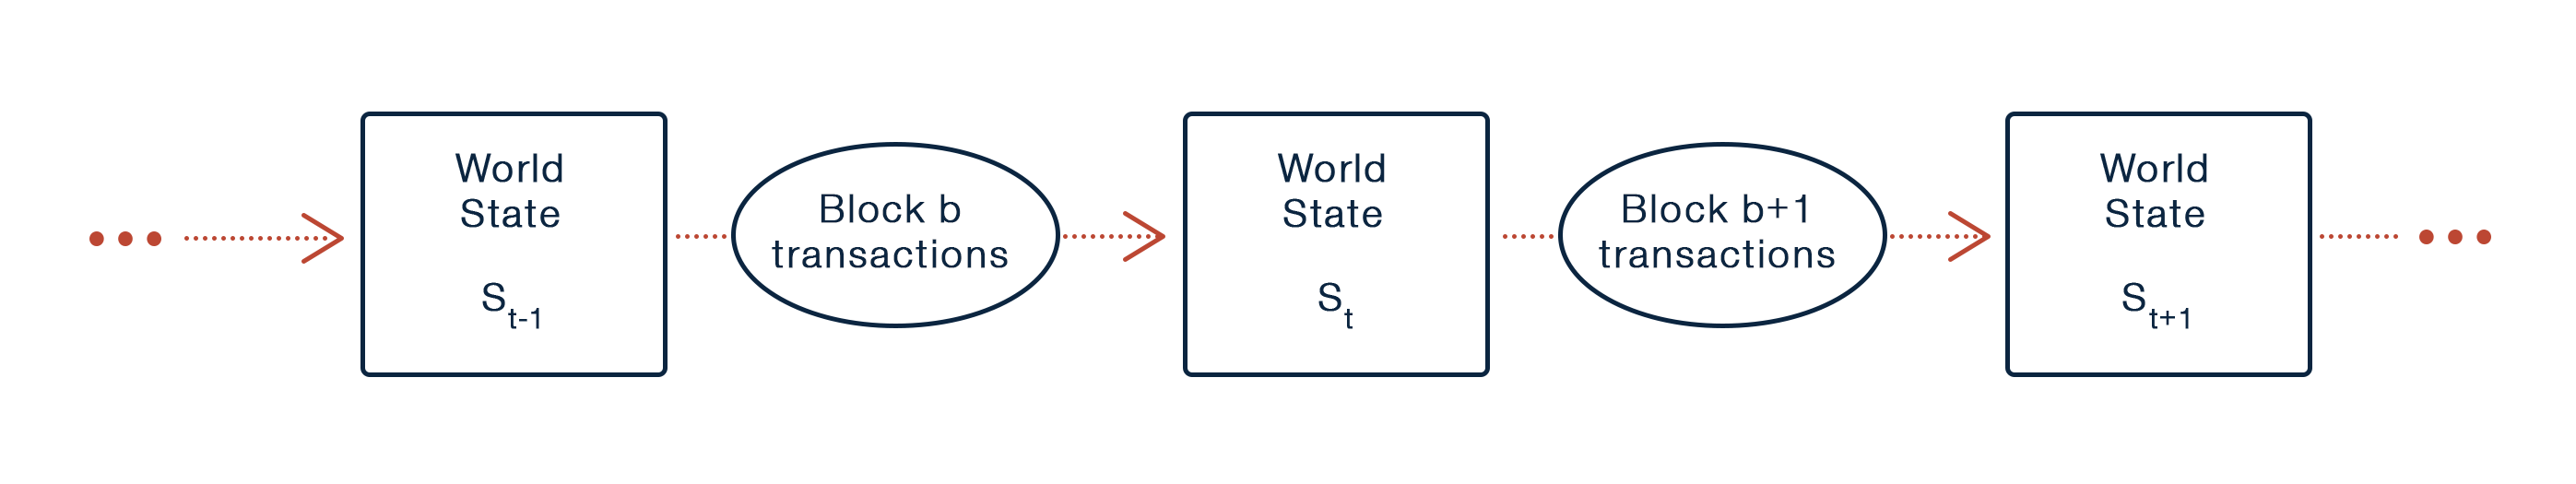
\includegraphics[scale=0.1]{assets/figures/blockchain-world-state}
\end{frame}

\note{
	Πριν περάσουμε στην ανάλυση του δεύτερου επιπέδου, θα κάνουμε μία σύντομη εισαγωγή στο blockchain.
	Το blockchain είναι μία σχετικά νέα τεχνολογία, η οποία περιγράφηκε για πρώτη φορά το 2008, αποτελώντας τη βάση του κρυπτονομίσματος Bitcoin.
	
	Με λίγα λόγια πρόκειται για μία δημόσια, αποκεντρωμένη και αμετάβλητη ως προς το ιστορικό της βάση δεδομένων.
	Είναι δημόσια, επειδή τα δεδομένα της μπορούν να διαβαστούν από όλους και οποιοσδήποτε μπορεί να δημιουργήσει έναν λογαριασμό και να συναλλάσσεται με αυτήν. Οι λογαριασμοί δημιουργούνται με διαδικασίες ασύμμετρης κρυπτογραφίας, χρησιμοποιώντας ως διεύθυνση το παραγόμενο δημόσιο κλειδί, όπως φαίνεται και στη διαφάνεια.
	
	Επιπλέον, το blockchain είναι αποκεντρωμένο, επειδή  αρχιτεκτονικά είναι ένα P2P δίκτυο, ή αλλιώς ένα δίκτυο ομότιμων κόμβων. Έτσι, δεν υπάρχουν servers και άρα αρχιτεκτονικά δεν υπάρχει κάποιο κεντρικό σημείο αποτυχίας. Δηλαδή δεν απαιτείται να εκχωρήσουμε κάπου εμπιστοσύνη - λειτουργεί όπως λέμε με trustless τρόπο.
	
	Επίσης, είναι μία βάση αμετάβλητη ως προς το ιστορικό της, δηλαδή ό,τι γράφεται δεν ξεγράφεται. Αυτό κατοχυρώνεται κρυπτογραφικά και κάνει τα δεδομένα αυθεντικά και επαληθεύσιμα: ανά πάσα στιγμή ανατρέχουμε στα προηγούμενα block και εξετάζουμε τις συναλλαγές, βλέπουμε τις ψηφιακές τους υπογραφές, κτλ.
	
	Όπως φαίνεται και στο σχήμα, πρόκειται τεχνικά για μία μηχανή καταστάσεων βασισμένη σε συναλλαγές. Δηλαδή μία αλυσίδα που μεγαλώνει συνεχώς με κάθε νέο block συναλλαγών, παράγοντας μία νέα κατάσταση.
	
	Τέλος, θα πρέπει να πούμε ότι στις συναλλαγές υπάρχουν τέλη. Αυτά τα τέλη τα παίρνουν οι κόμβοι που συμμετέχουν στη διαδικασία εξόρυξης των κρυπτονομισμάτων και είναι απαραίτητα γιατί διασφαλίζουν το δίκτυο από επιθέσεις, ενώ ταυτόχρονα αποτελούν ένα οικονομικό κίνητρο για να συμμετάσχει κάποιος σε αυτό.
}